\section{Related Work}
% 
\begin{figure*}
	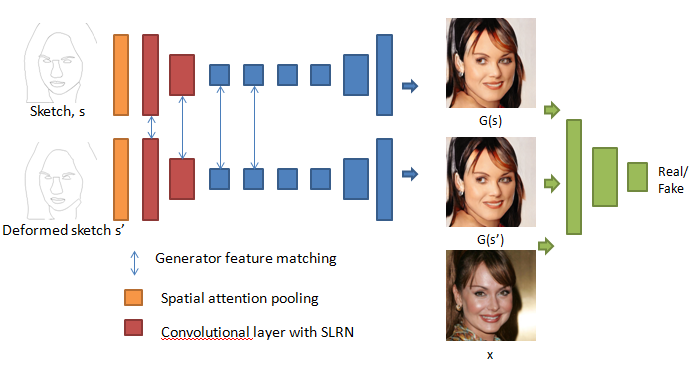
\includegraphics[width=\textwidth]{figs/architecture.png}
	\caption{The architecture of our model.}
	\label{fig:architecture}
\end{figure*}
%
\subsection{Image-to-Image Translation}
Given an input image from one domain, an image-to-image translation model outputs a corresponding image from another domain and preserves the content in the input image. Existing image-to-image translation models are based on generative adversarial networks conditioned on images. 
%
Pix2pix~\cite{pix2pix} is the first general image-to-image translation model which is able to be applied to different scenarios according to the paired training images, such as, semantic maps to real images, day images to night images, image coloring, and edge maps to real images. 
%
\cite{outdoor_scene} utilizes semantic label maps and attributes of outdoor scenes as input and generates the corresponding photo-realistic images.
%
In order to model multi-modal distribution of output images, BicycleGAN~\cite{BicycleGAN} encourages the connection between the output and the latent code to be invertible.
%
CycleGAN~\cite{CycleGAN}, DualGAN~\cite{DualGAN}, and DiscoGAN~\cite{DiscoGAN} propose unsupervised image translation model with a similar idea named cycle consistency borrowed from language translation literature. 
%
StarGAN~\cite{StarGAN} presents a framework for one-to-many image translation by adding a domain code as input and a domain classifier as guidance.
%
Pix2pixHD~\cite{pix2pixHD} is proposed as a high-resolution image-to-image translation model for generating photo-realistic image from semantic label maps using a coarse-to-fine generator and a multi-scale discriminator. It can also be applied to edge-to-photo generation by using the paired edge maps and photos as training data.
%
\td{However, xxxxxxxxxxxxxx}

\subsection{Sketch-based Image generation}
Sketch-based image generation is a hot topic in computer vision and computer graphics. Given a sketch of a scene with text labels for objects, traditional methods, such as Sketch2Photo~\cite{Sketch2Photo} and PhotoSketcher~\cite{PhotoSketcher}, search corresponding image patches from a large image dataset and then fuse the the retrieved image patches together according to the sketch. These methods are not able to ensure the global consistency of the resultant image and fails to generate totally new images.
%
After the breakthrough made by deep neural networks (DNN) in computer graphics and computer vision, a variety of DNN-based models have been proposed for sketch-based image generation. 
%
The general image-to-image translation models mentioned above are able to be applied to sketch-based image generation once sketches and the corresponding images are used as training data.
%
Besides, many other models are designed specially for sketch inputs. SketchyGAN~\cite{SketchyGAN} aims to generate real images from multi-class sketches. A novel neural network module, called mask residual unit (MRU), is proposed to improve the information flow by injecting the input image at multiple scales. \td{Edge maps are extracted from real images and utiled as training sketches.} However, the resultant images of SketchyGAN are still not satisfied.
%

\subsection{pooling}

\subsection{Face Generation and Editing}

\td{All existing methods for local face editing require the user to provide masks and strokes manually}. In comparison, strokes are only the input to indicate the desired shape. Our system automatically interprets the intended edit and produces the local change accurately. This greatly reduces users' burden and preserves the fluency of user interaction. 

\td{Only local edit in a relatively small area is supported.} As reported in SC-FEGAN~\cite{}, artifacts appear when complete a large region in FaceShop~\cite{}.
